\section{Procedure}
\label{sec:procedure}
In the following section an overview about the optical instruments is given. The important parts are
\begin{itemize}
  \item A laser as a source for coherent light (Part 2),
  \item The beam collimator (Part 4),
  \item a biconvex lens (Part 5),
  \item the Nd:YAG crystal with mirroring coating (Part 6),
  \item a resonator mirror (Part 7),
  \item a KTP crystal which is capable of SHG (Part 10).
\end{itemize}
For easier operation and measurements, a target (Part 9) and filter unit (Part 8) are used as well. 
In \autoref{fig:setup} the arrangement of the optical parts is shown, the mentioned numbers
correspond to what has been used in the manual and the figure thereof \cite{elas_manual}.
\begin{figure}
    \centering
    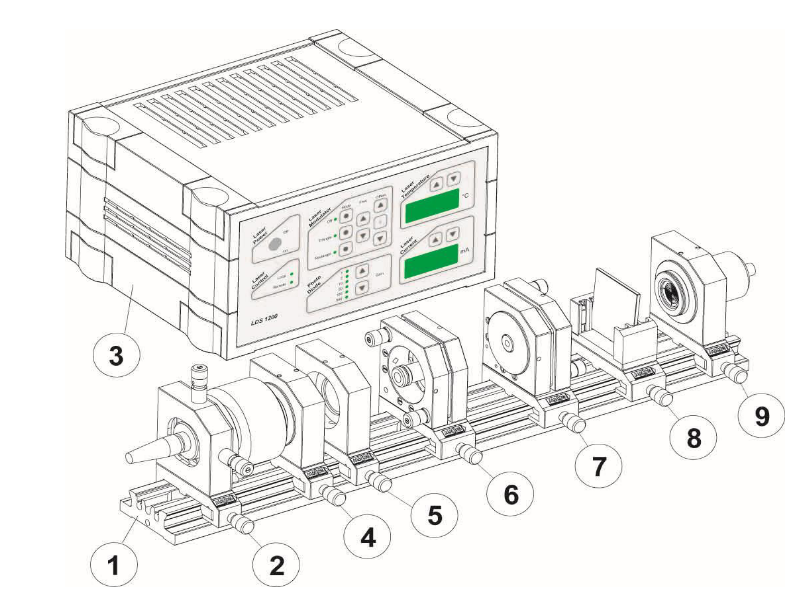
\includegraphics[width=0.4\textwidth]{media/Setup.png}
    \caption{Setup and Components of the experiment \cite{elas_manual}. Since this is a general
    picture, the KTP crystal (part 10) is missing.}
    \label{fig:setup}
\end{figure}
The parts not mentioned yet are the power supply (Part 3) and the mounting rail (Part 1).

For the exact procedure one can consult the manual, the main steps are as follows:
\begin{enumerate}
  \item Add the laser (2), target (9) and collimator (4) to the rail (1), adjusting 
    the collimator such that the laser is focused on the target screen,
  \item place the biconvex lens (5) between collimator (4) and screen (9),
  \item adjust the the Nd:YAG resonator (6) such that the crystal section is in line with the beam
    and place it after the biconvex.
  \item place the second resonator mirror (7) between (6) and (9), with a similar adjustment
    regarding the mirror angling. Furhter more, place the filter unit (8) with an RG1000 filter in
    front of the target. This step creates an optical cavity which will be used for the SHG.
  \item place the KTP crystal (10) between (7) and (6).
\end{enumerate}
Most important here is the fine tuning for each component, which are done in accordance with the
manual, an infrared detection card can be helpful.

Also one should make sure that he or she follows the safety advices regarding the laser, as it can
damage your eye and burn surfaces.
